\documentclass[12pt]{article}
\usepackage[utf8]{inputenc}
\usepackage{graphicx}
\usepackage{float}
\usepackage{subcaption}
\usepackage[style=ieee]{biblatex}
\usepackage{multicol}
\usepackage{fullpage}
\usepackage{amsmath}
\usepackage[font = small, labelfont = bf]{caption}

\addbibresource{paper_citations.bib}

\title{Feline Leukemia Virus transmission in Iberian Lynx population}
\author{Agathe Yvinec Tolmer, Thomas Rimbot, Pranav Sadana}
\date{April 2020}

\begin{document}

\maketitle

\begin{quote}
    {\textbf{Abstract:}}
 We combined two models -the SIR model for disease dynamics modified to take into account inter-species transmission, and the Rosenzweig-MacArthur for population dynamics, modified to look at prey-mesopredator-predator relations- to study the case of a Feline Leukemia Virus (FeLV) outbreak within the rabbits-cats-lynx system in the Doñana Park in Spain. We performed sensitivity analysis of the parameters in order to determine the cause of infection in the lynx population, looked into different possible scenarios and performed stability analysis of equilibrium to study the system's behaviour. Finally, we described and compared different conservation measures to prevent the lynxes from extinction. The results suggest that the transmission of FeLV from cats to lynxes leads to an outbreak in the lynx population. Moreover, the most effective measure to prevent an outbreak is to vaccinate the lynxes against FeLV. The paper highlights that mesopredators play an important role in disease dynamics of apex predators and not only in the predator - prey dynamics. 
\end{quote}
\vfill\eject

\tableofcontents

\vfill\eject
\section{Introduction}
\quad The Iberian lynx, \emph{Lynx pardinus}, is the most endangered feline species in the world. It is found in Spain and Portugal and 20 years ago, its population was as small as 100 adult individuals in total. This was partly due to the main prey of the Iberian lynx, the European rabbit, \emph{Oryctolagus cuniculus}. During the second half of the 20th century, the European rabbit suffered from diseases like rabbit haemorrhagic disease which contributed to its decline. Since then, the remaining lynx populations have been protected and some individuals were reintroduced, leading to a total of 475 Iberian lynxes in 2017\cite{noauthor_iberian_nodate}.\\

\quad The Iberian lynx is known to compete with cats (\emph{Felis sp.}) for preys and cats killed by lynxes are frequently reported. In 2007, an epidemic of Feline Leukemia Virus (FeLV) struck one of the populations of Iberian lynxes in Doñana, Spain. Out of approximately 50 lynxes, 12 got infected and 7 died within a year\cite{meli_feline_2010}. The virus was contracted by contact with infected cats, and then likely spread inside the lynx population. \\

\quad The Feline Leukemia Virus is a retrovirus affecting the Felidae family, commonly called felids. It is mostly transmitted by exchange of blood and saliva, which happens a lot for felids during grooming or fights involving biting. The virus is highly infectious, but a fraction of infected carry the matching antibodies and thus develop immunity. These immune individuals cannot spread the virus to susceptibles. For individuals who become persistently infected, FeLV provokes a generalized infection of the blood and immune system cells, which causes the cats to be more susceptible to other infections. As there is no known cure yet, the infected felids eventually die of overwhelming infections.\\
 
\quad Finally, in 2017, conservation researchers monitoring the Iberian lynx population came across the first case of a lynx consuming a cat\cite{najera_lynx_2019}. Since cats also consume European rabbits, our 3 animals are linked by a trophic web of the shape Predator (lynx) – Mesopredator (cat) – Prey (rabbit).\\

\quad Since the Iberian lynx population is already at risk of extinction, an epidemic of FeLV could be a big concern for conservation specialists. Therefore in this project, we plan to investigate two major questions:
\begin{itemize}
    \item \textbf{How does the FeLV spread to lynxes: does it spread more through lynx-cat interactions or lynx-lynx interactions?}
    \item \textbf{How to protect the lynx population: which conservation measures could be implemented and how efficient would they be?}
\end{itemize}

\section{Model}
\quad Similar models already exist but not for this particular situation. Moreover, most models are either of the form Prey-Mesopredator-Predator without disease or Prey-Predator with disease. So we basically combined these two into one. There are two main dynamics to model: population and disease dynamics. For population dynamics, we used the Rosenzweig-MacArthur model, and for the disease the SIR model.

\quad In this section we describe the model we implemented. From now on, we denote the populations by L (Lynxes), C (Cats) and R (Rabbits).
\subsection{Assumptions}
\quad Several assumptions have been made, either because of a lack of information or for simplicity:
\begin{enumerate}
	\item Rabbit population is mostly constant and large. This is a big assumption because in reality, the population of the European rabbit is reduced due to the important epidemics it has faced in the past. We assumed this for simplicity and also to account for the other potential preys that are not included in our model. \cite{wave_of_chaos}
	\item Infection doesn't change hunting efficiency. That is, if an animal (lynx or cat) is infected, it is neither more or less efficient in hunting or in being hunted. This is assumed for simplicity, because FeLV infection has a variety of consequences and can also open the door to other infections, which makes it hard to blame specific symptoms on the virus.
	\item Lynxes cannot become naturally immune to the disease. While this is theoretically possible, there is a limited amount of information on FeLV epidemics in lynxes. We assume that they can recover without immunity, but otherwise they eventually die. \cite{meli_feline_2010}
	\item Cats do not attack lynxes. If a lynx attacks a cat, it results in the cat's death, thus there is no transmission of the virus from lynxes to cats.
	\item Finally, some assumptions have been made while estimating parameters. These will be detailed in the next sections.
\end{enumerate}
\subsection{Population Dynamics}
\quad At first, we wanted to use the prey-predator dynamics seen in class involving Lotka-Volterra equations and then extend it to take into account the mesopredator. But in the end we decided to use another version of this model: the Rosenzweig-MacArthur model. This choice has been made mainly for two reasons. Firstly, this is an extended and more accurate version of the Lotka-Volterra model. Secondly, some parameters for the population dynamics have been found in a paper that used this kind of model. \cite{wave_of_chaos} We also added a slight modification to this model.

\subsubsection{The Rosenzweig-MacArthur Model}
\quad In this part we explain the idea behind this model. Here is an example for a simple prey-predator dynamics with prey $x$ and predator $y$ (and parameters a, b, p, q):\\

$\frac{dx}{dt} = ax(1 - \frac{x}{\gamma}) -p\frac{xy}{1 + x}$

$\frac{dy}{dt} = q\frac{xy}{1 + x} - by$\\

\quad Two things are different from the usual model. First, the parameter $\gamma$ which is the carrying capacity of the environment for the prey. In the absence of predators, the prey population will grow, but not up to infinity. It stops at a certain threshold $\gamma$, which makes more sense biologically. Second, the interaction between $x$ and $y$ is no longer simply multiplicative, but divided by a term $x + 1$. This is so that the predation rates saturate when $x$ becomes very large.

\quad For these reasons, we used this model and adapted it to study the Prey-Mesopredator-Predator interactions.
\subsubsection{Modification}
\quad We also added a slight modification to this model so that it takes into account the carrying capacity of predators. As before, this makes more sense biologically (cats cannot grow up to infinity). The parameters for this are shown in the next subsection.
\subsubsection{Parameters}


\quad Most parameters come from estimations. This is mainly the case for cats parameters ($e_{CR}, e_{LC}, q_{L}, p_{C}$ etc.). We could not find a good source with parameters so we inferred them from lynx parameters, following the fact that cats need less food to grow more (because they are smaller, they will be a more efficient predator \cite{holt_alternative_2007}), and that lynxes eat cats very rarely. 

\quad For initial population values, we estimated $C_{0}$ to be around 500. Note that this is the sum of feral and domestic cat populations. While there are not many feral cats left (around 30 \cite{soto_navarro_surprising_2013}), the disease comes from domestic cats from neighbouring towns, and these cats are very numerous.

\quad Concerning carrying capacities, we inferred them from initial population values. The values for $K_{L}$ and $K_{R}$ are equal.

\begin{tabular}{|c|p{4cm}|c|c|c|}
	
	\hline
	Parameter & Definition & Estimate & Units & Source \\
	\hline
	$e_{LR}$ & Growth rate of lynxes thanks to rabbits consumed & 0.127 & Per day & \cite{wave_of_chaos} \\
	\hline
	$e_{CR}$ & Growth rate of cats thanks to rabbits consumed & 0.24 & Per day & \cite{soucy_cats_2017},Estimation \\
	\hline
	$e_{LC}$ & Growth rate of lynxes thanks to cats consumed & 0.0001 & Per day & Estimation \\
	\hline
	$q_{L}$ & Death rate of cats because of lynxes & 0.1 & Cat per lynx per day & Estimation \\
	\hline
	$p_{C}$ & Death rate of rabbits because of cats & 0.5 & Rabbit per cat per day & \cite{soucy_cats_2017},Estimation \\
	\hline
	$p_{L}$ & Death rate of rabbits because of lynxes & 0.5 & Rabbit per lynx per day & \cite{wave_of_chaos} \\
	\hline
	$x_{L}$ & Death rate of lynxes without prey & 0.12 & Per day & \cite{wave_of_chaos} \\
	\hline
	$x_{C}$ & Death rate of cats without prey & 0.08 & Per day & Estimation\\
	\hline
	$y_{R}$ & Growth rate of rabbits & 6.1 & Per day & \cite{wave_of_chaos} \\
	\hline
	$K_{L}$ & Carrying capacity of environment for lynxes & 800 & Lynx & Estimation \\
	\hline
	$K_{C}$ & Carrying capacity of environment for cats & 800 & Cat & Estimation \\
	\hline
	$K_{R}$ & Carrying capacity of environment for rabbits & 1500 & Rabbit & Estimation \\
	\hline
	$L_{0}$ & Initial lynx population & 30 & Lynx & \cite{meli_feline_2010} \\
	\hline
	$C_{0}$ & Initial cat population & 500 & Cat & Estimation \\
	\hline
	$R_{0}$ & Initial rabbit population & 800 & Rabbit & Estimation \\
	\hline
\end{tabular}	\\\\

\subsubsection{Equations}
\quad Using these parameters, we get the following equations for population dynamics:
\begin{itemize}
    \item $\frac{dL}{dt} = e_{LC}\frac{CL}{C + 60}(1 - \frac{L}{K_{L}}) + e_{LR}\frac{RL}{R + 48}(1 - \frac{L}{K_{L}}) - x_{L}L$
    \item $\frac{dC}{dt} = e_{CR}\frac{CR}{R + 48}(1 - \frac{C}{K_{C}}) - q_{L}\frac{CL}{C + 60} - x_{C}C$
    \item $\frac{dR}{dt} = y_{R}R(1 - \frac{R}{K_{R}}) - p_{C}\frac{CR}{R + 48} - p_{L}\frac{RL}{R + 48}$
\end{itemize}
\quad Note that what changes is the values 48 and 60 that appear in the prey-predator interactions. They represent the extent to which the environment provides protection to the prey \cite{wave_of_chaos}.

\subsection{Disease Dynamics}
\quad To model the disease dynamics, we chose to use the SIR model seen in class. We modified it to match the dynamics of FeLV observed independently in cats \cite{fromont_modelling_1997} and lynxes \cite{meli_feline_2010}, and then connected the 2 systems. In this subsection, there will be no mention of the rabbits because they only take part in the population dynamics part of our model.
\subsubsection{The SIR Model}
\quad The SIR model is a compartmental model for disease dynamics where we separate the population in 3 compartments: Susceptibles, Infected and Recovered. The basic equations are as follows: \\

$\frac{dS}{dt} = -\beta SI$

$\frac{dI}{dt} = \beta SI - \gamma I$

$\frac{dR}{dt} = \gamma I$\\


\quad $\beta$ represents the infection rate of the disease, which is the probability that a susceptible meets an infected, multiplied by the probability of transmitting the disease when a contact occurs. $\gamma$ is the recovery rate of infected individuals.

\subsubsection{Modification}
\quad We added several modifications to the basic SIR model to match our situation. First, since there is no recovery from FeLV for cats but there can be immunity, we used the Recovered compartment for the immune cats. That is, when a cat gets infected, it will move on to the Recovered compartment if it is immune to FeLV. If it is not, the cat stays in the Infected compartment.\cite{fromont_modelling_1997} Then, since we assume there is no immunity for lynxes, we used a SIS model instead. Thus when a lynx recovers, it goes back to the Susceptible compartment. Finally, to account for the fact that the disease spreads from cats to lynxes, we added an infection term in the lynx model. Infected lynx are not only created by interactions between a susceptible and an infected lynx, but also by interactions between an infected cat and a susceptible lynx.

\subsubsection{Parameters}

\begin{tabular}{|c| p{6cm}|c|c|c|}
	
	\hline
	Parameter & Definition & Estimate & Units & Source \\
	\hline
	$\beta_{L}$ & Number of interactions infected lynx-lynx leading to infection & 0.0027 & Lynx per day & Estimation \\
	\hline
	$\beta_{C}$ & Number of interactions infected cat-cat leading to infection & 0.015 & Cat per day & Estimation \\
	\hline
	$\beta_{CL}$ & Number of interactions infected cat-lynx leading to infection & 0.002 & Lynx per day & Estimation \\
	\hline
	$\gamma_{L}$ & Recovery rate for lynxes & 0.00011 & Per day & \cite{meli_feline_2010} \\
	\hline
	$\rho_{C}$ & Recovery rate for cats & 0.00046 & Per day & \cite{fromont_modelling_1997} \\
	\hline
	$\delta_{L}$ & Death rate of lynxes because of disease & 0.0032 & Per day & \cite{meli_feline_2010} \\
	\hline
	$\delta_{C}$ & Death rate of cats because of disease & 0.0007 & Per day & \cite{fromont_modelling_1997} \\
	\hline
	init\_infected & Fraction of initially infected cats & 0.03 & $\emptyset$ & Estimation\\
	\hline
\end{tabular} \\\\


\quad Note that the parameters $\beta$'s are not exactly the same as in the usual SIR model. This is because they are supposed to depend on the population size. In the SIR model, the population is constant so that they are constant too. But in our model, since we consider population dynamics as well, the population is not constant. In general, infection rates are computed this way:\\

infection rate = $\frac{number \ of \ interactions \ with \ individuals \ * \ fraction \ of \ infections}{population}$. 
\\

In our case, consider the infection rate between infected cats and lynxes:
\\

infection rate = $\frac{number \ of \ lynxes \ encountered  \ * \ fraction \ of \ infections}{Lynx \ population}$ = $\frac{\beta_{CL}}{L}$
\\

\quad Now as for their values, they once again mainly come from estimations, information on this matter being really scarce. Here we show our reasoning and assumptions used to compute $\beta_{CL}$:

\begin{itemize}
    \item The lynx population is estimated to be around 30 individuals in a 250 000 $km^{2}$ area. Therefore the lynx density is $\frac{30}{250 000}$. 
    \item A cat moves in a 5*5 km square everyday, so it would be in the same 1*1 km square as $25 * \frac{30}{250 000}$ lynxes.
    \item If a cat and a lynx are in the same 1*1 km square, they meet with probability 0.7 (the cat can escape or the lynx can not kill it), which gives us a total of $0.7 * 25 * \frac{30}{250 000}$ interactions between an infected cat and the lynx population.
    \item If the lynx kills the cat, it has a 0.95 probability of becoming infected (infection by blood/saliva). So in the end our value for $\beta_{CL}$ is $0.95 * 0.7 * 25 * \frac{30}{250 000} = 0.002$
\end{itemize}

\quad This clearly has some flaws in it but we could not find any data for it.

\subsubsection{Equations}
\quad Using these parameters, we get the following equations for disease dynamics:
\begin{itemize}
    \item $\frac{dS_{L}}{dt} = \gamma_{L}I_{L} - \beta_{L}I_{L}\frac{S_{L}}{L} - \beta_{CL}I_{C}\frac{S_{L}}{L}$
    \item $\frac{dI_{L}}{dt} = \beta_{L}I_{L}\frac{S_{L}}{L} + \beta_{CL}I_{C}\frac{S_{L}}{L} - \gamma_{L}I_{L} - \delta_{L}I_{L}$
    \item $\frac{dS_{c}}{dt} = -\beta_{C}I_{C/}\frac{S_{C}}{C}$
    \item $\frac{dI_{C}}{dt} = \beta_{C}I_{C}\frac{S_{C}}{C} - \rho_{C}I_{C} - \delta_{C}I_{C}$
    \item $\frac{dR_{C}}{dt} = \rho_{C}I_{C}$
\end{itemize}
\quad Note that each $\beta$ term is divided by the total population size of the relevant animal to account for the fact that the usual $\beta$ parameters in SIR models depend on population size.

\subsection{Final Model}

\quad Figure 1 shows a diagram summarizing the model. We have 6 compartments, so 6 equations, with 23 parameters.\\
\begin{figure}[!ht]
    \centering
    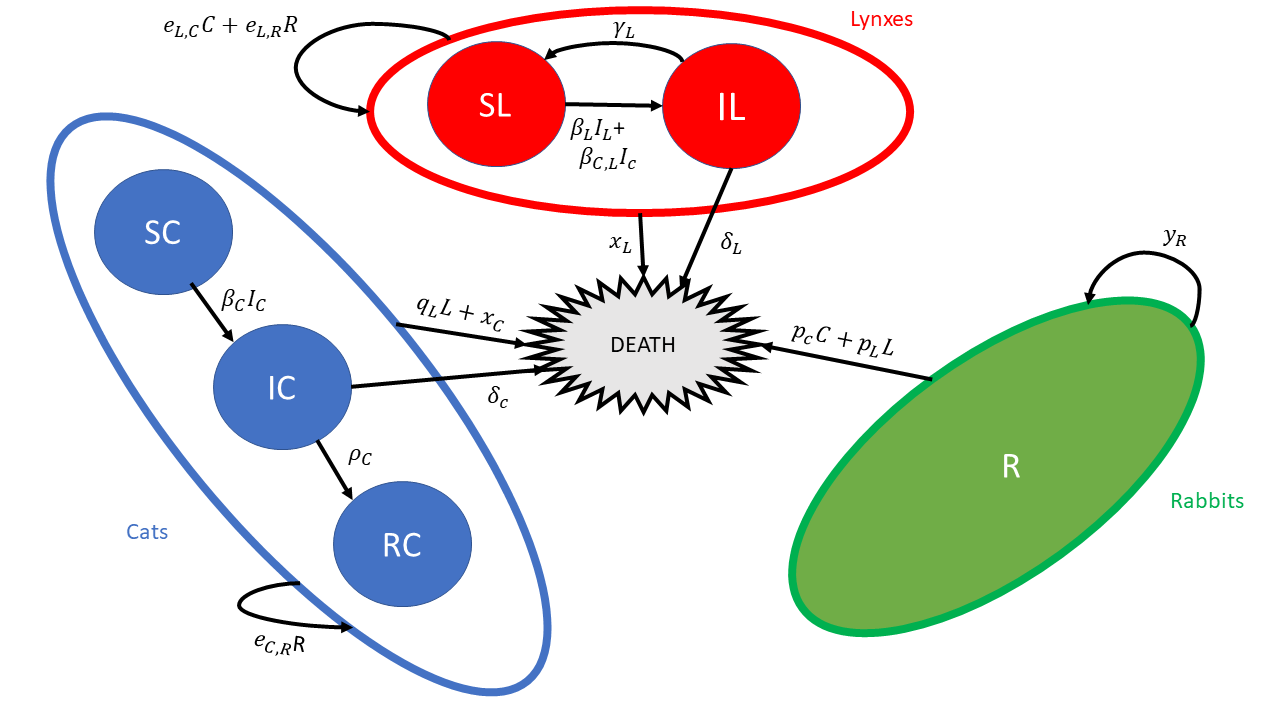
\includegraphics[width = \textwidth]{images/graph.png}
    \caption{The coupled population and disease dynamics of the Lynx- Cat - Rabbit system.}
    \label{fig:my_label}
\end{figure}


\quad Combining the equations for the population and disease dynamics, we get the final equations:

\begin{itemize}
	\item $\frac{dS_{L}}{dt} = [e_{LC}\frac{CS_{L}}{C + 60}(1 - \frac{L}{K_{L}}) + e_{LR}\frac{RS_{L}}{R + 48}(1 - \frac{L}{K_{L}}) + \gamma_{L}I_{L}] - [x_{L}S_{L} + \beta_{L}I_{L}\frac{S_{L}}{L} + \beta_{CL}I_{C}\frac{S_{L}}{L}]$
	\item $\frac{dI_{L}}{dt} = [e_{LC}\frac{CI_{L}}{C + 60}(1 - \frac{L}{K_{L}}) + e_{LR}\frac{RI_{L}}{R + 48}(1 - \frac{L}{K_{L}}) + \beta_{L}I_{L}\frac{S_{L}}{L} + \beta_{CL}I_{C}\frac{S_{L}}{L}] - [x_{L}I_{L} + \gamma_{L}I_{L} + \delta_{L}I_{L}]$
	\item $\frac{dS_{c}}{dt} = [e_{CR}\frac{RS_{C}}{R + 48}(1 - \frac{C}{K_{C}})] - [q_{L}\frac{S_{C}L}{C + 60} + x_{C}S_{C} + \beta_{C}I_{C}\frac{S_{C}}{C}]$
	\item $\frac{dI_{C}}{dt} = [e_{CR}\frac{RI_{C}}{R + 48}(1 - \frac{C}{K_{C}})  + \beta_{C}I_{C}\frac{S_{C}}{C}] - [q_{L}\frac{I_{C}L}{C + 60} + x_{C}C + \rho_{C}I_{C} + \delta_{C}I_{C}] $
	\item $\frac{dR_{C}}{dt} = [e_{CR}\frac{RR_{C}}{R + 48}(1 - \frac{C}{K_{C}}) + \rho_{C}I_{C}] - [x_{C}R_{C} + q_{L}\frac{R_{C}L}{C + 60}]$
	\item $\frac{dR}{dt} = [y_{R}R(1 - \frac{R}{K_{R}})] - [p_{C}\frac{CR}{R + 48} + p_{L}\frac{RL}{R + 48}]$
\end{itemize}
Where $L = S_{L} + I_{L}$, $C = S_{C} + I_{C} + R_{C}$.

\subsection{Conservation Models}
\quad We chose to look at 3 different conservation models: isolation of infected lynxes, control of the cat population and vaccination of susceptible lynxes. For each one, we used our final model and added a few modifications to express the effect of the conservation measure.

\subsubsection{Lynx Isolation}
\quad To model the isolation of infected lynx from the rest of the population, we added a compartment for isolated lynxes. Infected lynxes are transferred to this compartment at a rate $isol_{L}$. Isolated lynxes die of FeLV at the same rate as the rest of the infected population, but have a higher chance of recovering and going back to susceptibles, denoted $cure_{L}$. We added to this model the fact that quarantined lynxes can be treated by the conservation specialists, which increases their chance of recovering. Therefore for this conservation measure, the equations are as follows (using $Q_{L}$ to denote quarantined lynxes). 

\begin{itemize}
	\item $\frac{dS_{L}}{dt} = [e_{LC}\frac{CS_{L}}{C + 60}(1 - \frac{L}{K_{L}}) + e_{LR}\frac{RS_{L}}{R + 48}(1 - \frac{L}{K_{L}}) + \gamma_{L}I_{L} + cure_{L}Q_{L}] - [x_{L}S_{L} + \beta_{L}I_{L}\frac{S_{L}}{L} + \beta_{CL}I_{C}\frac{S_{L}}{L}]$
	\item $\frac{dI_{L}}{dt} = [e_{LC}\frac{CI_{L}}{C + 60}(1 - \frac{L}{K_{L}}) + e_{LR}\frac{RI_{L}}{R + 48}(1 - \frac{L}{K_{L}}) + \beta_{L}I_{L}\frac{S_{L}}{L} + \beta_{CL}I_{C}\frac{S_{L}}{L}] - [x_{L}I_{L} + \gamma_{L}I_{L} + isol_{L}I_{L} + \delta_{L}I_{L}]$
	\item $\frac{dQ_{L}}{dt} = isol_{L}I_{L} - [cure_{L}Q_{L} + \delta_{L}Q_{L}]$
	\item $\frac{dS_{c}}{dt} = [e_{CR}\frac{RS_{C}}{R + 48}(1 - \frac{C}{K_{C}})] - [q_{L}\frac{S_{C}L}{C + 60} + x_{C}S_{C} + \beta_{C}I_{C}\frac{S_{C}}{C}]$
	\item $\frac{dI_{C}}{dt} = [e_{CR}\frac{RI_{C}}{R + 48}(1 - \frac{C}{K_{C}})  + \beta_{C}I_{C}\frac{S_{C}}{C}] - [q_{L}\frac{I_{C}L}{C + 60} + x_{C}C + \rho_{C}I_{C} + \delta_{C}I_{C}] $
	\item $\frac{dR_{C}}{dt} = [e_{CR}\frac{RR_{C}}{R + 48}(1 - \frac{C}{K_{C}}) + \rho_{C}I_{C}] - [x_{C}R_{C} + q_{L}\frac{R_{C}L}{C + 60}]$
	\item $\frac{dR}{dt} = [y_{R}R(1 - \frac{R}{K_{R}})] - [p_{C}\frac{CR}{R + 48} + p_{L}\frac{RL}{R + 48}]$
\end{itemize}
\quad For our simulation, we chose $isol_{L} = 0.01$ which represents 1 lynx quarantined every 100 days or approximately 3 months. 

\subsubsection{Cats Control}
\quad To model a control of the cat population, we simply changed the initial population size and carrying capacity of the environment for cats. In reality, this could be achieved with a reduction of the feral cat population of the area, and a total isolation of infected domestic cats. That way, less cats are actually present in our area of study.

\quad For our simulations, we chose to place the initial population size and the carrying capacity at 50 cats. 

\subsubsection{Lynx Vaccination}
\quad Finally to implement the vaccination of susceptible lynxes, we added a compartment to the model for vaccinated lynxes. They answer to the same population dynamics as the susceptible lynxes but cannot get infected. This adds one new parameter, $vac_{L}$, which is the percentage of the susceptible lynxes that are vaccinated in one day. The equations for the cat and rabbit populations stay the same. Thus the equations for this conservation measure are: 
\begin{itemize}
    \item $\frac{dS_{L}}{dt} = [e_{LC}\frac{CS_{L}}{C + 60}(1 - \frac{L}{K_{L}}) + e_{LR}\frac{RS_{L}}{R + 48}(1 - \frac{L}{K_{L}}) + \gamma_{L}I_{L}] - [x_{L}S_{L} + \beta_{L}I_{L}\frac{S_{L}}{L} + \beta_{CL}I_{C}\frac{S_{L}}{L} + vac_{L}S_{L}]$
	\item $\frac{dI_{L}}{dt} = [e_{LC}\frac{CI_{L}}{C + 60}(1 - \frac{L}{K_{L}}) + e_{LR}\frac{RI_{L}}{R + 48}(1 - \frac{L}{K_{L}}) + \beta_{L}I_{L}\frac{S_{L}}{L} + \beta_{CL}I_{C}\frac{S_{L}}{L}] - [x_{L}I_{L} + \gamma_{L}I_{L} + \delta_{L}I_{L}]$
	\item $\frac{dS_{c}}{dt} = [e_{CR}\frac{RS_{C}}{R + 48}(1 - \frac{C}{K_{C}})] - [q_{L}\frac{S_{C}L}{C + 60} + x_{C}S_{C} + \beta_{C}I_{C}\frac{S_{C}}{C}]$
	\item $\frac{dV_{L}}{dt} = e_{LC}\frac{CV_{L}}{C + 60}(1 - \frac{L}{K_{L}}) + e_{LR}\frac{RV_{L}}{R + 48}(1 - \frac{L}{K_{L}}) + vac_{L}S_{L} - x_{L}V_{L}$
	\item $\frac{dI_{C}}{dt} = [e_{CR}\frac{RI_{C}}{R + 48}(1 - \frac{C}{K_{C}})  + \beta_{C}I_{C}\frac{S_{C}}{C}] - [q_{L}\frac{I_{C}L}{C + 60} + x_{C}C + \rho_{C}I_{C} + \delta_{C}I_{C}] $
	\item $\frac{dR_{C}}{dt} = [e_{CR}\frac{RR_{C}}{R + 48}(1 - \frac{C}{K_{C}}) + \rho_{C}I_{C}] - [x_{C}R_{C} + q_{L}\frac{R_{C}L}{C + 60}]$
	\item $\frac{dR}{dt} = [y_{R}R(1 - \frac{R}{K_{R}})] - [p_{C}\frac{CR}{R + 48} + p_{L}\frac{RL}{R + 48}]$
\end{itemize}
\quad We ran our model with $vac_{L} = 0.01$, which represents 1 lynx vaccinated every 100 days. We chose this low value to account for the fact that to vaccinate a lynx, conservators first need to catch it, test it to see if it is infected with FeLV and then vaccinate it, so the process might take a while. 

\section{Results}

\subsection{Main Model Output}
\begin{figure}[!ht]
    \centering
    \begin{subfigure}{0.45\textwidth}
        \centering
        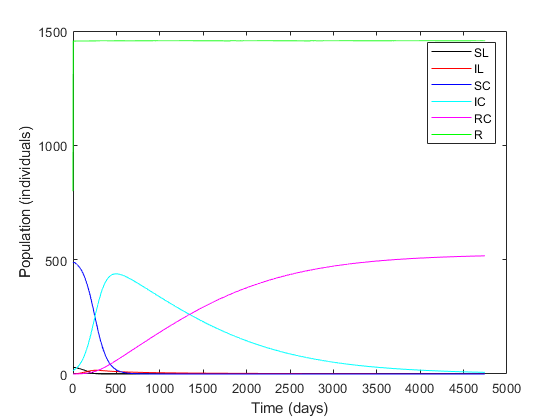
\includegraphics[width=\textwidth]{images/main_all.png}
        \caption{All compartments}
    \end{subfigure}
    \begin{subfigure}{0.45\textwidth}
        \centering
        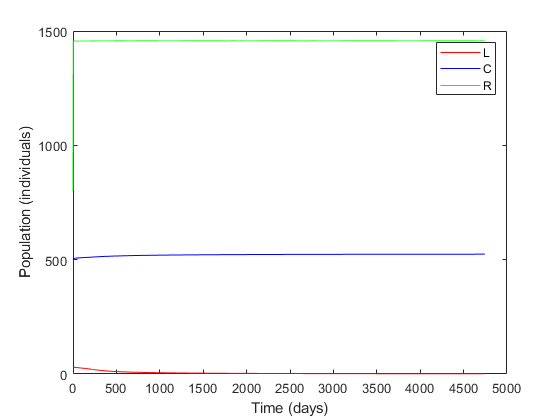
\includegraphics[width=\textwidth]{images/main_total.png}
        \caption{Total population of each animal}
    \end{subfigure}\\
    \begin{subfigure}{0.45\textwidth}
        \centering
        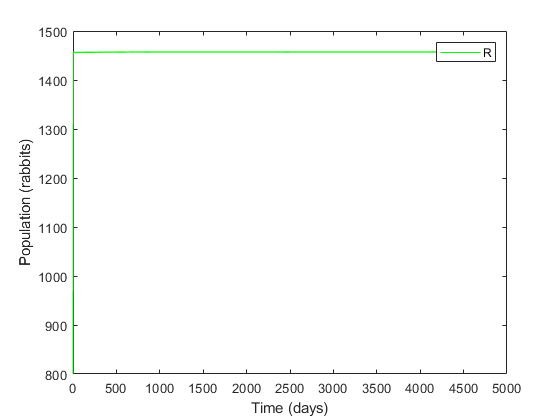
\includegraphics[width=\textwidth]{images/main_R.png}
        \caption{Rabbit population}
    \end{subfigure}
    \begin{subfigure}{0.45\textwidth}
        \centering
        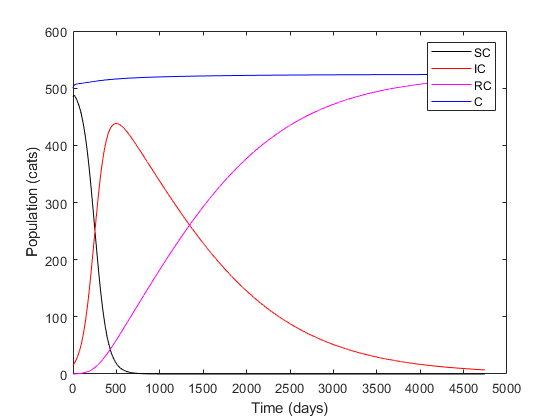
\includegraphics[width=\textwidth]{images/main_C.png}
        \caption{Cat population}
    \end{subfigure}\\
    \begin{subfigure}{0.45\textwidth}
        \centering
        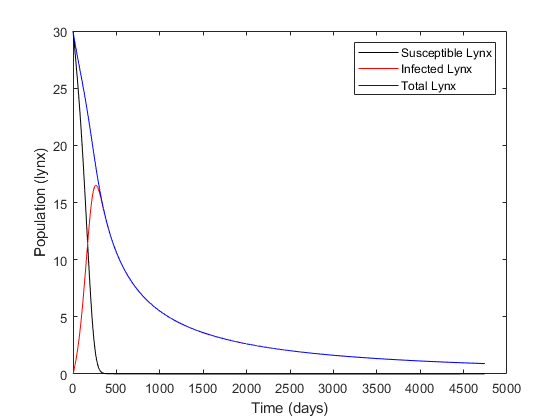
\includegraphics[width=\textwidth]{images/main_L.png}
        \caption{Lynx population}
    \end{subfigure}
    \begin{subfigure}{0.45\textwidth}
        \centering
        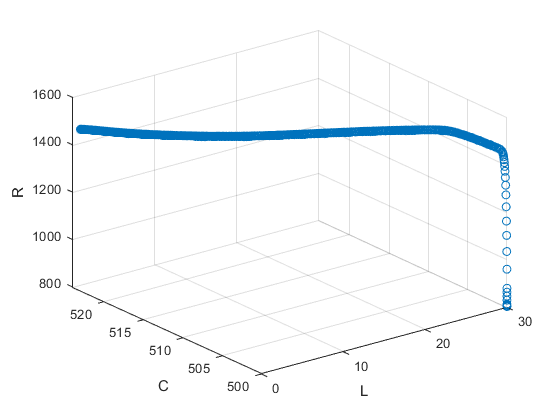
\includegraphics[width=\textwidth]{images/main_phase.png}
        \caption{Phase diagram}
    \end{subfigure}
\caption{Outputs of the main model}
\end{figure}

\quad The outputs of our main model can be seen in Figure 2. First, we note that the populations of cats and rabbits are large and stable. In the cat population, there was a outbreak of FeLV with the peak of infection happening after about 2 years. Then the infection dies down. Throughout the simulation, the number of immune cats goes up steadily until they make up almost the whole population. 

\quad Then regarding the lynx population, we calculated the basic reproductive number for the infection in lynxes using the two transmission rates: (1) between the cats and the lynxes and (2) within the lynx population.  The basic reproductive number for FeLV for lynxes was 1.47. Since $R_0 > 1$, we would expect the infection to lead to an epidemic, and we see in Figure 2 that it is the case. The lynxes get rapidly infected before 500 days of the beginning of the outbreak. By then, we note a rapid exponential decline in the lynx population. The population goes extinct within 4000 days of the outbreak.


\subsection{Stability Analysis }

\quad Disease and population dynamics usually have very different equilibria (stable I=0 for SIR and unstable periodic for Lotka-Volterra). The Rosenzweig Mac-Arthur model has a bit of a mix: the points in the phase plane spiral towards an equilibrium point. Since we combined these two approaches, we thought it would be interesting to perform an analysis of the ODEs to find and classify equilibria. \\

\quad Since the system is non-linear, we had to use linearization around an equilibrium point:

$X^{*} = [0 \ 0 \ 524.6 \ 0 \ 0 \ 1457.2]$. 

This point has been computed with Matlab's $fsolve $ starting from a guess $X_{0} = [0 \ 0 \ 0.5 \ 525 \ 0 \ 0 \ 1458]$. It corresponds to an equilibrium situation between cats and rabbits after the disease is gone, without lynxes. \\

\quad Then, using Matlab's $jacobian$, we computed the Jacobian of the system and evaluated it at $X^{*}$, then computed its eigenvalues. These are shown in this vector:
$
\begin{bmatrix}
    -0.000052 \\ 0.00056\\ 0.0021\\ 0.014\\ -0.15\\ -5.75
\end{bmatrix}
$\\

\quad As we can see, no eigenvalues has real part 0, and some are positive, therefore this equilibrium is unstable. This comes from the population dynamics. The main explanation is that this equilibrium doesn't have any infected animal ($X^{*}(2) = X^{*}(4) = 0$). So what happens if we add for example 0.1 susceptible lynx? They will thrive (as any superpredator), not killed by the disease and grow exponentially away from equilibrium. Below is a graph of 10 simulations of the lynx population, each being a 5 years run from the equilibrium plus a little perturbation ranging from 0 to 1 susceptible lynx added. We can see that it clearly moves far from $X^{*}$, confirming its instability.

\begin{figure}[!ht]
    \centering
    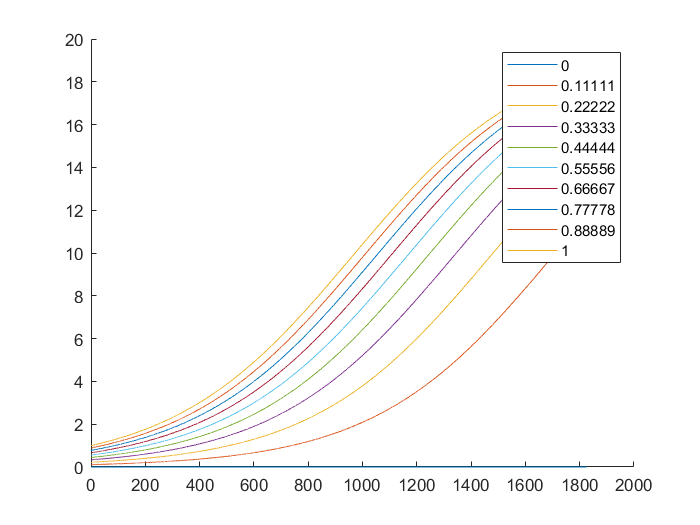
\includegraphics[scale=0.75]{images/stability.png}
    \caption{Lynx population during 5 years after perturbation from the equilibrium}
    \label{fig:my_label}
\end{figure}

\quad Note that this is a very interesting result in terms of conservation: if an epidemic of FeLV is detected in the park, it could be a good idea to transfer healthy individuals into a non-infected environment until the epidemic is completely stopped in the park (at this point we would be at equilibrium). Then, reintroducing these individuals will allow them to grow and expand the lynx population without fear of the disease.

\subsection{Sensitivity Analysis}
\quad To estimate the impact of each of the transmission rates on the transmission of FeLV in lynxes, we compared the sensitivity of the model to the transmission parameters for  (1) between cats and lynx $\beta_{CL}$ and (2) within the lynx population $\beta_L$. The model sensitivity of transmission of FeLV from cats to lynx was -0.0713, while the sensitivity of transmission of FeLV within the lynx population was -0.0084. The model was not highly sensitive to both the transmission parameters as the sensitivity values were low. However, the sensitivity value for the transmission from cats to lynx was ten times higher than the transmission between the lynx population. 

\subsection{Conservation Measures}
To explore the efforts to control disease spread, we considered three conservation measures (1) quarantining individual lynx who are infected, (2) controlling the population of feral cats, and (3) vaccinating the susceptible lynx.


\subsubsection{Lynx Isolation}
\quad When we isolate lynxes at a rate of 1 infected lynx every 100 days, we get the population dynamics for the lynx population shown in Figure 4.

\begin{figure}[!ht]
    \centering
    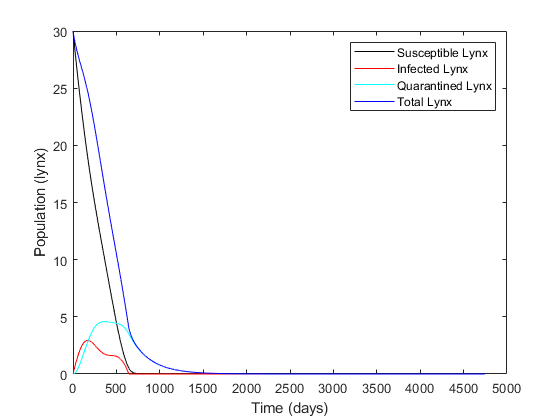
\includegraphics[scale=0.75]{images/isolation.png}
    \caption{Population dynamics of lynxes with 1 lynx quarantined/100 days}
    \label{fig:my_label}
\end{figure}

\quad When the infected lynx are quarantined individually, the model suggests that lynx population declines rapidly. Although the lynxes do not get severely infected, the population goes extinct within 1500 days of the outbreak. This is likely because the way we constructed the model implies that quarantined lynxes do not reproduce. Therefore as long as they are in isolation, they cannot sustain the population; and we see on our graph that after approximately 2 years, the remaining lynx population is entirely made up of quarantined individuals. 


\subsubsection{Cats Control}
\quad When we limit the number of cats in the protected area to 50, we get the population dynamics for the lynx population shown in Figure 5.

\begin{figure}[!ht]
    \centering
    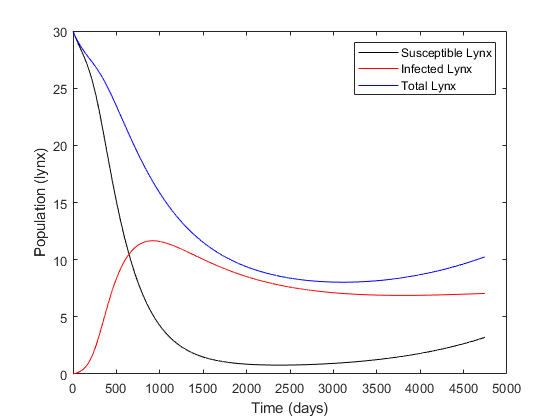
\includegraphics[scale=0.75]{images/catcontrol.png}
    \caption{Population dynamics of lynxes with at most 50 cats in the area}
    \label{fig:my_label}
\end{figure}

\quad We see that the total lynx population drops down to approximately 10 individuals and then seems to grow again. We ran the stimulation for a longer time (8000 days, i.e. 20 years) and the population keeps growing, with a decrease of infected individuals. Therefore this seems to be a good outcome, but on the other hand, the cat population starts to decrease because of the large number of lynxes. This is could become a problem since in this situation, the cat population of the area is already limited to only 50 individuals.

\subsubsection{Lynx Vaccination}
\quad With a vaccination rate of one lynx every 100 fays, we get the results for the dynamics of the lynx population as shown in Figure 6.

\begin{figure}[!ht]
    \centering
    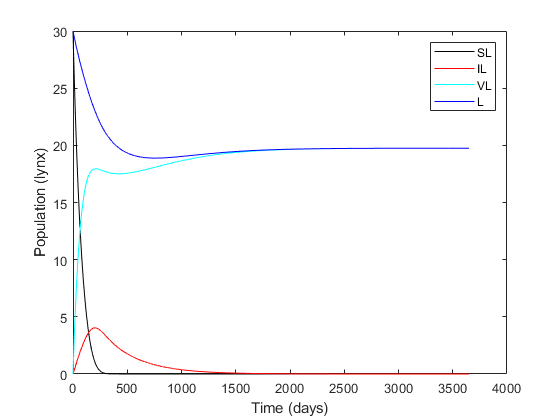
\includegraphics[scale=0.75]{images/vaccination.png}
    \caption{Population dynamics of lynxes with 1 lynx vaccinated every 100 days}
    \label{fig:my_label}
\end{figure}

\quad When the susceptible lynxes are vaccinated once every 100 days, the infection can be controlled and the virus can be eradicated in 2000 days (~5 years). The population recovers from the infection and stabilizes to around 20 individuals who are vaccinated against the virus. This is good because it means that as long as the virus doesn't mutate and renders the vaccine ineffective, the lynx population will not suffer from a new FeLV epidemic.



\section{Discussion}

\quad Our model provides the population dynamics of the lynx population under an outbreak of FeLV originating from the cat population in the same region. The model along with our parameter estimations suggest that the infection of FeLV into the lynx population will lead to a deadly epidemic. Exploring disease control measures for the lynx population, vaccination is the most effective way of saving the lynx population out of the three conservation measures implemented during the 2007 outbreak.\cite{lopez_management_2009}  

\quad The lynx population is affected by transmission from both cats and other lynxes. The model suggests that there is more transmission of FeLV  from cats to lynxes rather than transmission within the lynx population. The greater effect of transmission from cats to lynxes indicates that, with respect to the transmission of FeLV in lynx, the cats act as a reservoir of the virus and interactions between lynxes and cats can lead to outbreaks in the lynx population. However, the model overall was not highly sensitive to both the transmissions. This insensitivity of the model  may have led us to consider a longer time frame for the outbreak. The lynx population may actually go extinct sooner than the model predicts.\\

\quad We considered three conservation measures (1) quarantining infected lynx, (2) controlling the population of cats within the protected area, and (3) vaccinating susceptible lynxes. Between the first two conservation measures, controlling cat population was a more effective manner of saving the lynx population which was also highlighted by the relatively larger sensitivity of the model to the transmission of FeLV from cats to lynx. Moreover, when the lynxes are isolated, their reproductive possibilities reduce which drives the population extinct sooner than the infection itself.  

\quad The model suggests that the best method to save lynxes is vaccinating them. Vaccinating helps the population recover in number and helps stabilize the population which has also been strongly argued for in past studies \cite{meli_feline_2010}\cite{lopez_management_2009}. Even with a modest capture and vaccination rate of just 1 lynx every 100 days, the measure is the most effective. However, the model assumes that a vaccination gives lifelong immunity. In reality, the vaccinations used for the lynx are the same as the cats and require booster shots to provide strong immunity \cite{lopez_management_2009}.  Keeping track of vaccination booster shots in a wild population may be difficult. However, higher rates of captures and vaccinations have been shown to be possible during the 2007 outbreak \cite{lopez_management_2009}. A higher vaccination rate may not only prevent infection once, but regular vaccination may prevent future outbreaks. \\
 


\quad Our model highlights the need to take preventative conservation actions such as vaccination against FeLV and controlling cat populations within protected areas. However, the model is based on mostly estimated parameters. Further studies need to be performed to collect empirical data so as to enhance the understanding of disease dynamics of FeLV in the lynx and improvement in model predictions. Such enhancements may improve precision of the outbreak timelines. The model also needs to account for animal behaviour and natural history of the lynx. For instance, male lynx are more prone to fighting during breeding season over access to mates\cite{mattisson_lethal_2013} which may lead to a higher spread of disease through males of the population. Moreover, the lynx population and the rabbit population have both been decimated due to habitat destruction and a disease in the rabbits.\cite{wave_of_chaos} Therefore, future studies need to account for the fragility of the small size of the population and the functional extinction of the population to enhance the understanding of the implications of the disease dynamics of such outbreaks. 





\section{Response to Questions From Presentation}

\quad In this section, we answer questions that have been asked during and after the presentation.

\begin{itemize}
    \item Are the cats wild or domestic and does it matter?\\
    When we estimated the total population size for the cats, we accounted for feral cats and domestic cats in the area. However, there is little information on disease dynamics of FeLV in feral cats since they are much more complicated to obtain than for domestic cats. Thus the disease dynamics are based on studies conducted on domestic cats. We don't think this is a problem because the domestic cat population is more than 10 times bigger than the feral cats' in our simulation. 
    \item Considering the small number of lynxes, is a continuous model appropriate?\\
    We thought about this question when designing the model but for simplicity we decided to still use a continuous model. Moreover, the numbers of cats and rabbits are large so for these populations the continuous model makes sense. But we acknowledge the fact that our predictions on the population size of lynxes would be more precise with a discrete model.
    \item Are 1000s of days the correct timescale for an FeLV epidemic?\\
    We decided to use this timescale because the natural life expectancy of a lynx is 13 years (~5000 days). This way we can see if with the disease our lynx population dies off faster than it would with no disease. Concerning the timescale of the actual disease, we only had one main source describing the FeLV epidemic in the Doñana population, so we used the information of this paper to infer our parameters. In our results, we see on the graphs that most of the disease dynamics occur in the first 2 years, which seems to match the observations of our source.
    \item Based on our model, which conservation measure would we recommend?\\
    According to our model, the most efficient conservation measure would be vaccinating the lynxes. We see that it is the measure that allows the lynx population to stabilize at the highest value. For an even better efficiency, we could also advise conservation specialist to combine the vaccination method with the cats control, which also seemed to have a good effect on the lynx population survival.
\end{itemize}

\section{Contributions of Each Group Member}
\quad We all contributed equally to the power point presentation.

\subsection{Agathe Yvinec Tolmer}
\begin{itemize}
    \item Provided the necessary background and biological knowledge
    \item Parameter research
    \item Introduction, response to questions and contributed to section 2.1, 2.3, 2.5, and 3 of the report
    \item Bibliography
\end{itemize}
\subsection{Thomas Rimbot}
\begin{itemize}
    \item Parameter research and estimations
    \item Implemented the code for basic model and conservation measures
    \item Ran simulations to debug the model
    \item Stability analysis of the equilibrium
    \item Abstract and contributed to section 2 and 3.2 of the report
\end{itemize}
\subsection{Pranav Sadana}
\begin{itemize}
    \item Modelling background: developing the disease dynamic models (SIS, SISV)
    \item Sensitivity analyses and biological implications of the model and its parameters
    \item Discussion, conclusion and contributed to section 3 of the report
\end{itemize}
\section{Conclusion}
\quad This paper combines a predator-prey dynamics model, the Rosenzweig-MacArthur Model, with a disease dynamics model, SIR model. The coupling of the two models was then applied to a Predator - Mesopredator - Prey situation.  The model was used to explore the transmission of the Feline Leukemia Virus (FeLV) in the lynx population of a protected area of Doñana, Spain, through the mesopredators, cats. Our results suggest that the transmission of FeLV from cats to lynx would lead to an epidemic outbreak. We also highlight the effectiveness of preventative measures of vaccination, as well as the role of mesopredators in disease dynamics of endangered apex predators which may be applied to other similar systems.

\vfill\eject
\printbibliography

\end{document}
